\section{Shared memory paralelization avec numba}

Étant donné que Numba est une méthode d’implémentation de la parallélisation en mémoire partagée, ce qui est proposé est de remplacer par \texttt{prange} les boucles dans lesquelles chacune des itérations correspond au résultat d’un corps distinct et qui écrivent dans des positions éloignées du tableau, afin d’éviter des phénomènes comme les blocages dus à la synchronisation, qui pourraient affecter la qualité des résultats de la parallélisation initiale. En suivant cette idée, il est proposé d’implémenter la parallélisation avec mémoire partagée (\textit{Numba}) pour le calcul en plusieurs threads de l’accélération des corps ; pour cela, le décorateur est défini à \texttt{true} et, en outre, \texttt{range} est remplacé par \texttt{prange}. La parallélisation avec mémoire partagée n’est pas implémentée dans le calcul de la grille, car la présence de structures qui sont partagées, comme c’est le cas de \texttt{cell\_counts}, \texttt{current\_counts} et \texttt{body\_indices}, pourrait donner lieu à des problèmes de synchronisation dans la mémoire partagée et à une dégradation des résultats du calcul.

\begin{figure}[htbp]
\centering
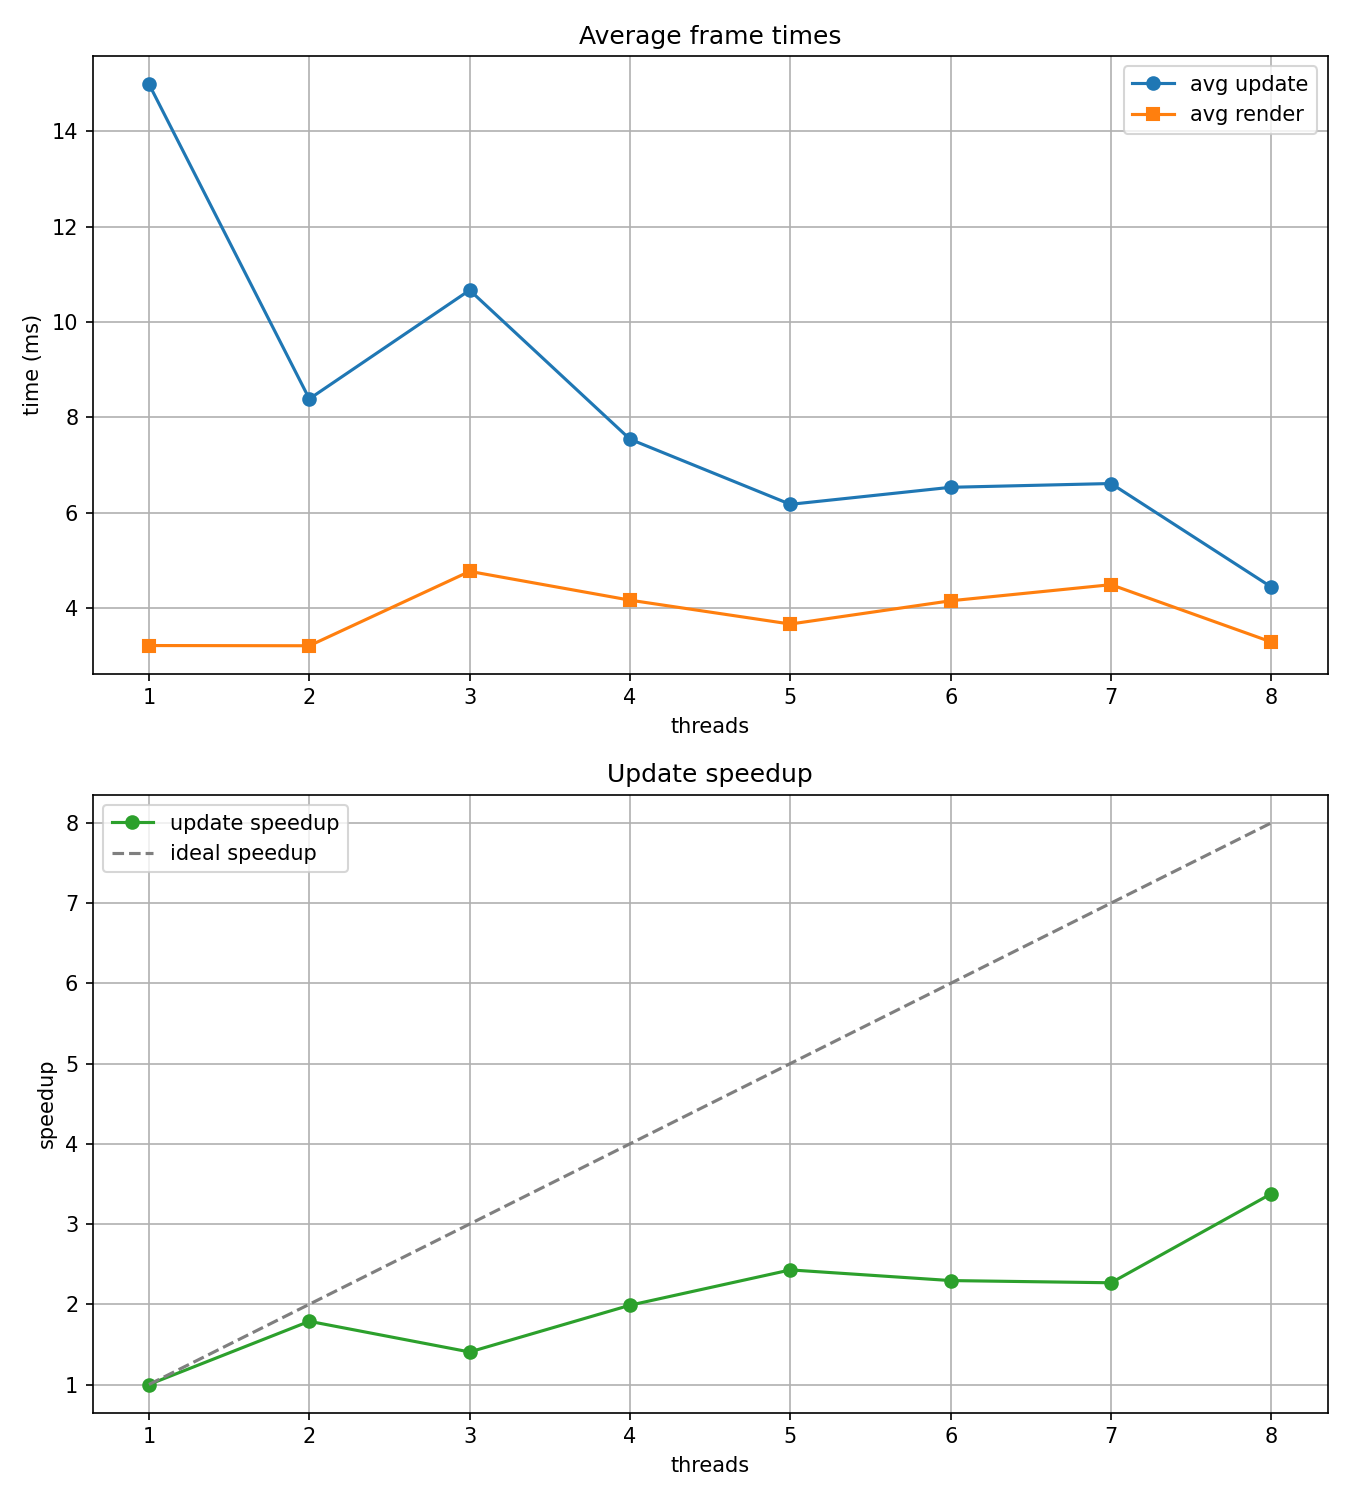
\includegraphics[width=\linewidth]{images/numba_parallel_timings.png}
\caption{Temps moyens de rendu et de mise à jour, ainsi que l’accélération obtenue en fonction du nombre de threads Numba.}
\label{fig:numba_parallel_timings}
\end{figure}


Les résultats montrent la diminution du temps moyen de rendu à mesure que l’on augmente le nombre de threads de calcul dans lesquels est répartie la boucle principale pour l’accélération de chaque corps. Néanmoins, on peut constater que le degré d’amélioration du temps de traitement à partir du deuxième thread s’éloigne du \textit{speedup} idéal, ce qui peut être lié aux effets de synchronisation de la mémoire partagée, aux limitations imposées par les sections du code qui ne sont pas parallélisables, ou encore au fait que la dynamique de la grille n’a pas été modifiée en utilisant Numba, étant donné que la nature de ses accès mémoire ne la rendait pas idéale pour cette implémentation.